%\section{Microprocessor}

\indent At the core of the sensor package is the microprocessor. The
microprocessor served as the data collection and distribution
device. The module received data from the peripheral devices and
either stored the data for further analysis or distributed it in
some manner. However, because of both the project requirements
and the diversity of the sensors, choosing the right
microprocessor meant looking closely at all of the requirements
for operation. These requirements may be seen below. 
\subsection{Necessary Specifications}
\subsubsection{Power Consumption}

\indent Though power was not a focus of this semester, the
microprocessor of choice was to be used through the next semester
as well. This means the module of choice should be low power and
made for embedded applications. 

\subsubsection{Timing Accuracy and Synchronization}

\indent Another important area to consider is the ability to time
synchronize with a central clock. This was also not a concern for
the prototyping stage this semester but the same board will be used
for the coming semester. In some way it must be feasible for the
computer chosen to communicate with a clock source and
synchronize itself. This could mean communicating with an
external GPS module or with a remote NTP server. 
\subsubsection{Sampling Frequency}

The microprocessor must be able to sample data from peripheral sensors at a rate fast enough to avoid aliasing data. Analysis from the Finite Element Modeling team was used to decide on this parameter

\subsubsection{Input Output Capabilities}

In order for the processor to collect and relay data from many
different sensors, there are strict input output needs. To
communicate with the Analog to Digital Converter (ADC), the
computer needs to have an Inter-Integrated Circuit ($I_2C$) bus.
Two Universal Asynchronous Receiver/Transmitter (UART) buses are
needed to communicate with the GPS module and a wireless
transmitter that has not been determined yet.

\subsubsection{Data Logging}

For testing, the ability to store data to a log file instead of
exporting via wireless was desired. This allowed testing of the
prototype without the use of wireless communications. The data
could be collected and simply stored for later analysis. 


\subsubsection{Software Development}

The platform chosen should a reasonably tested development
environment and SDK. The platform chosen should have a compiler
that makes use of popular languages. It should also be clear, if
more than one language may be used, what the advantages and
disadvantages of each approach would be. For instance, compiling
an executable vs executing a python script. 

\subsection{Platform Options}

\subsubsection{Microprocessor Comparison Table}
\begin{table}
\centering
\begin{tabular}{|l| p{3cm} | p{3cm} |}
\hline
\textbf{Microprocessor:} & BeagleBone Black 
%	\begin{figure}
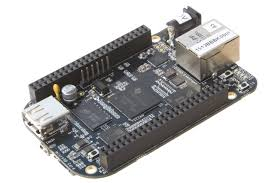
\includegraphics[scale = 0.25]{BeagleBoneBlack_Image.jpg}
%	\end{figure}
& Netburner MOD5270
%	\begin{figure}
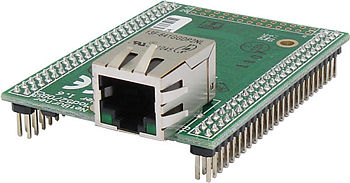
\includegraphics[scale = 0.25]{Netburner_MOD5270_Image.jpg}
%	\end{figure}
\\
\hline
\textbf{Clock Rate:}		&1GHz ARM Cortex-A8& 145.7MHz 
Freescale ColdFire 5270 \\
\hline
\textbf{I/O Pins:}		& 65  &46\\
\hline
\textbf{Power Consumption:}&	1.05-2.3 W @ 5V	& 1.65 W @ 3.3V	\\
\hline
\textbf{Data Storage:}	&			microSD		&	microSD	\\
\hline
\textbf{Supported Communications:}&	I$^2$C, SPI, 3 Serial 
Ports		&I$^2$C, QSPI, 3 Serial Ports		\\
\hline
\textbf{Software Development}&Python,C/C$^{++}$&C/C$^{++}$\\
\hline
\end{tabular}
\caption{\textit{Comparison table of two microprocessors that 
were looked into for the embedded sensor package}}
\label{tab:uProcOptions}
\end{table}

\subsubsection{BeagleBone Black}
\label{subsec:BeagleBoneBlack}
\indent The BeagleBone Black is single board computer (SBC) that
runs a Linux operating system (Angstrom). The board is powered by a
TI AM3358 Sitara ARM Cortex-A8 Microprocessor. The core is 32 bit,
and can reach up to 1 GHz clock speeds. The board comes with a
plethora of pins. Included are two $I_2C$ buses, four UART
ports, and over 60 GPIO pins. There are also ground, 3.3V, and
5V pins to drive peripheral devices. \\

\indent The board runs full blown Linux and root access is
available. This means that development is possible with a variety
of languages from C++ to Java-script More importantly, there are
third party API (Application Programming Interface) libraries for
the all of the board's input and output written for both Python
and Java-script Both are high level languages and allow for
efficient code development and quicker testing of hardware
development. 

\subsubsection{Netburner MOD5270}
\label{subsec:MOD5270}
\indent The Netburner MOD5270 is a powerful embedded
micro-controller The drawing feature of this board is the inclusion
of a real time clock and its Real Time Operating System. It brings
predictable multitasking and timing. Furthermore, there is an
on-board SD card slot that can be used for real time data
logging. The processor is a 32-bit Freescale ColdFire 5270
running at 145.7 MHz. The on-board Direct Memory Access (DMA)
timers are optimal for timing the application and
synchronizing data transfers. There are two UARTs and an
$I_2C$ bus to go along with various General Purpose
Input/Output (GPIO) pins, including interrupt enabled pins
for external triggering if necessary. \\

\indent The board has a C++/C cross compiler. The System Development
Knowledge (SDK) is well documented and there are many examples for
various applications. The Netburner does not run a full operation
system. Instead, it runs a Real Time Operating System which
handle multitasking with priority levels and cycling. This is
much preferred to a full operating system for an embedded system
as it makes timing more precise and the processor more
efficient. However, the downside to the low level nature of
the board is the development difficulty. The development is
more difficult and takes more time and precision to
perfect. It is also more difficult to modify than a higher
level program running atop a traditional OS layer as seen
in the BeagleBone Black.

\subsection{Platform Decision}

The BeagleBone Black was the single board computer chosen for the
system. The system clock is fast enough to handle data at a rate of
1 kHz, the maximum sampling rate that was used for data
collection. Also, there are four serial buses, so the board was
able to receive data from the external GPS receiver module.
Importantly, the board allowed for fast development with the
Analog to Digital converter chosen. Development would have
been much slower if a different board had been chosen. The
board was chosen because of its ability to satisfy all of the
requirements for the microprocessor while allowing for
dynamic testing throughout the prototyping stage. 
